% Exact LaTeX recreation of the supplied Phase-1.pdf
% Compile with pdfLaTeX.

\documentclass[11pt,a4paper]{article}

\usepackage[a4paper,left=2.0cm,right=2.0cm,top=3.55cm,bottom=1.55cm]{geometry}
\usepackage[T1]{fontenc}
\usepackage{lmodern}
\usepackage{graphicx}
\usepackage{xcolor}
\usepackage{array}
\usepackage{tabularx}
\usepackage{ragged2e}
\usepackage{enumitem}
\usepackage{fancyhdr}
\usepackage{tikz}
\usetikzlibrary{positioning,arrows.meta,fit,backgrounds}
\usepackage{setspace}

% -------------------------------------------------
% COLOURS
% -------------------------------------------------
\definecolor{TitleBlue}{RGB}{61,103,154}

% -------------------------------------------------
% GENERAL SETTINGS
% -------------------------------------------------
\setlength{\parindent}{0pt}
\setlength{\parskip}{0pt}
\renewcommand{\arraystretch}{1.0}

\newcommand{\blueheading}[1]{%
    {\sffamily\color{TitleBlue}\fontsize{15}{18}\selectfont #1}%
}

\newcommand{\bluebigheading}[1]{%
    {\sffamily\bfseries\color{TitleBlue}\fontsize{16}{19}\selectfont #1}%
}


\newcommand{\answerbox}[2][3.0cm]{%
    \vspace{2pt}
    \noindent
    \fbox{%
        \begin{minipage}[t]{\dimexpr\textwidth-2\fboxsep-2\fboxrule\relax}
            \vspace{1mm}
            \normalfont #2
            \vspace{1mm}
        \end{minipage}
    }
}

\pagestyle{fancy}
\fancyhf{}
\renewcommand{\headrulewidth}{0pt}
\renewcommand{\footrulewidth}{0pt}

\fancyhead[L]{%
    \sffamily\bfseries\itshape\fontsize{10.5}{12}\selectfont
    DS(TCS-302) \& OOPs(TCS-7) 
}
\fancyhead[R]{%
    \sffamily\bfseries\fontsize{10.5}{12}\selectfont
    PROJECT PROPOSAL
}
\fancyfoot[R]{%
    \itshape\fontsize{10}{12}\selectfont
    Page \thepage
}
\setlength{\headheight}{14pt}
\setlength{\headsep}{23pt}
\setlength{\footskip}{24pt}

\begin{document}

\vspace*{4mm}

\bluebigheading{PROJECT AND TEAM INFORMATION}

\vspace{1cm}

\blueheading{Project Title}

\vspace{1mm}

\answerbox[1.3cm]{Hospital Patient Management System using Priority Queue, AVL Tree, and Hash-based Indexing}

\vspace{7mm}

\blueheading{Student / Team Information}

\vspace{2mm}

\noindent
\begin{tabularx}{\textwidth}{|>{\centering\arraybackslash}p{3.4cm}|>{\RaggedRight\arraybackslash}p{0.46\textwidth}|>{\RaggedRight\arraybackslash}X|}
\hline

\begin{minipage}[t][2.6cm][c]{\linewidth}
\vspace{1.5mm}
\textbf{Team member 1 (Team Lead)}\\[-1mm]
\end{minipage}

&
\begin{minipage}[t][2.6cm][c]{\linewidth}
\vspace{1.5mm}
\textit{Gaurav Gailakoti -- 2518342}\\
\textit{Section I}
\end{minipage}

&
\begin{minipage}[t][2.6cm][c]{\linewidth}
\centering
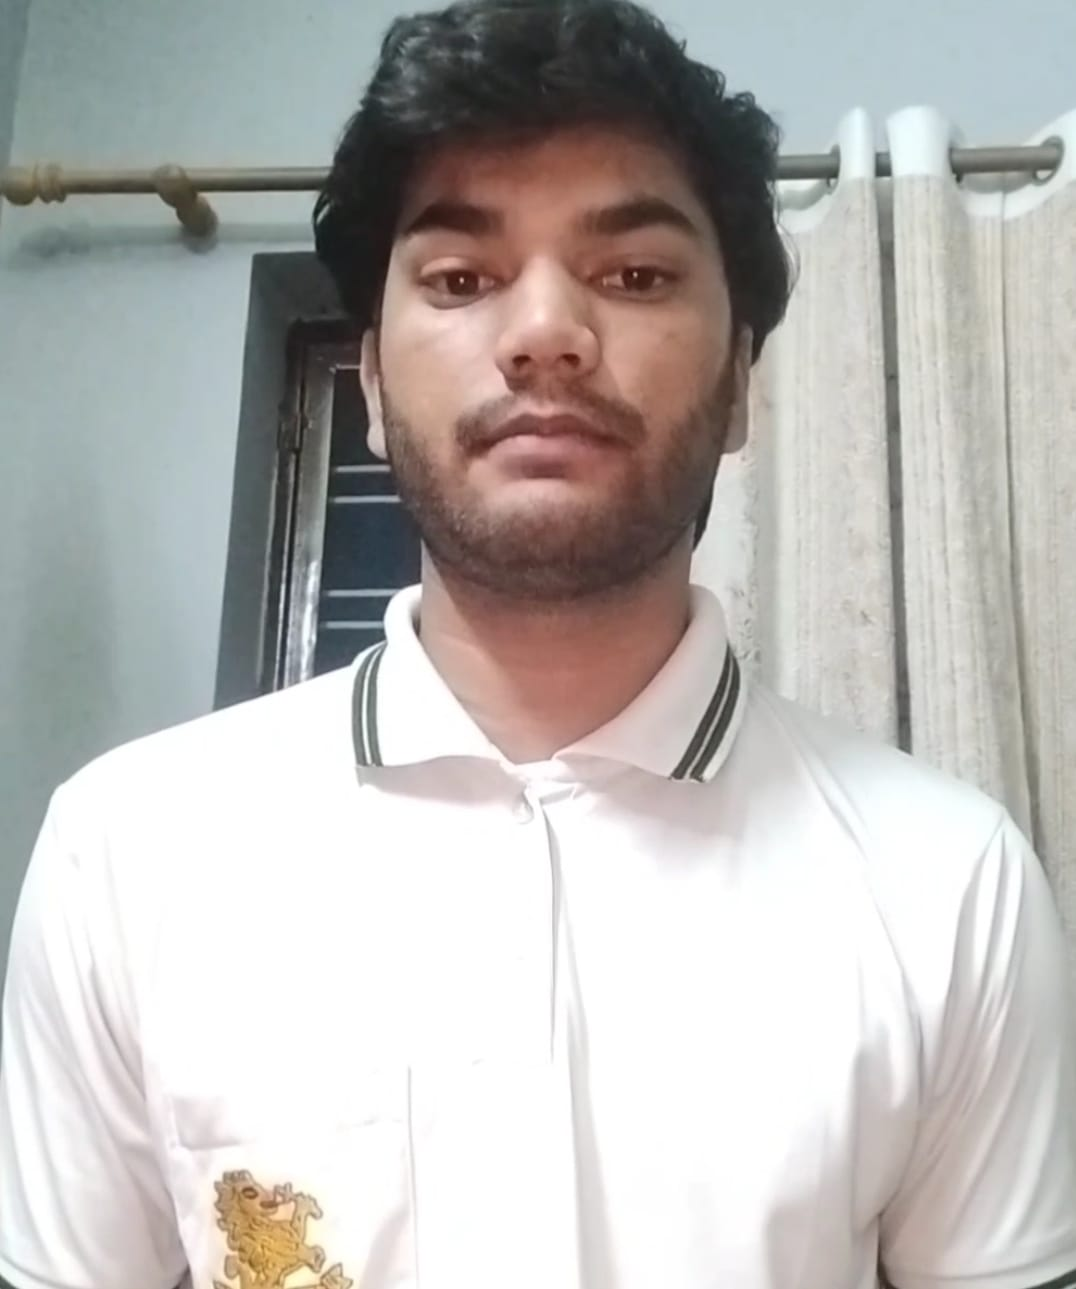
\includegraphics[width=2.0cm,height=2.3cm,keepaspectratio]{gaurav.jpeg}
\end{minipage}
\\
\hline

\begin{minipage}[t][2.6cm][c]{\linewidth}
\vspace{1.5mm}
\textbf{Team member 2}\\[-1mm]
\end{minipage}

&
\begin{minipage}[t][2.6cm][c]{\linewidth}
\vspace{1.5mm}
\textit{Atikur Rehman -- 2518774}\\
\textit{Section I}
\end{minipage}

&
\begin{minipage}[t][2.6cm][c]{\linewidth}
\centering
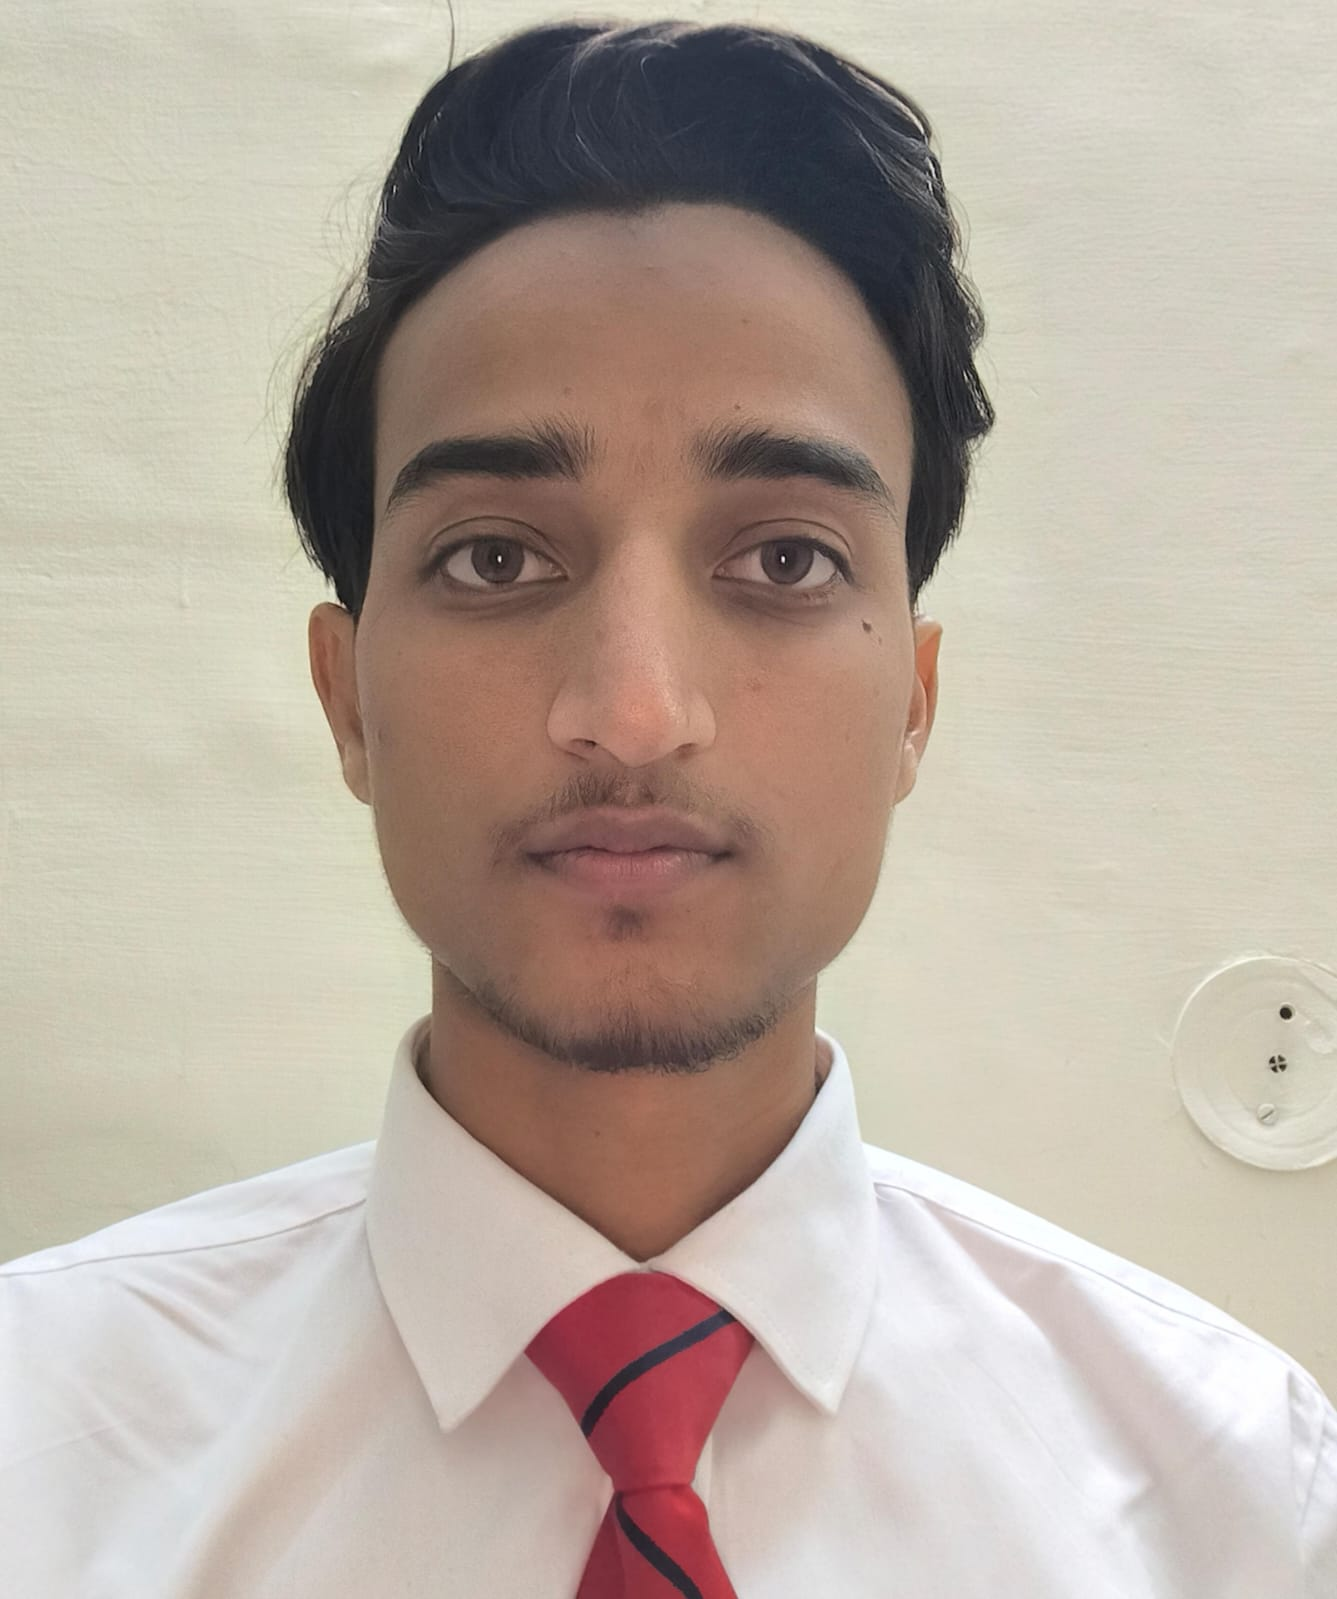
\includegraphics[width=2.0cm,height=2.3cm,keepaspectratio]{atikur.jpeg}
\end{minipage}
\\
\hline

\begin{minipage}[t][2.6cm][c]{\linewidth}
\vspace{1.5mm}
\textbf{Team member 3}\\[-1mm]
\end{minipage}

&
\begin{minipage}[t][2.6cm][c]{\linewidth}
\vspace{1.5mm}
\textit{Kartikey Thapliyal -- 2518398}\\
\textit{Section I}
\end{minipage}
&
\begin{minipage}[t][2.6cm][c]{\linewidth}
\centering
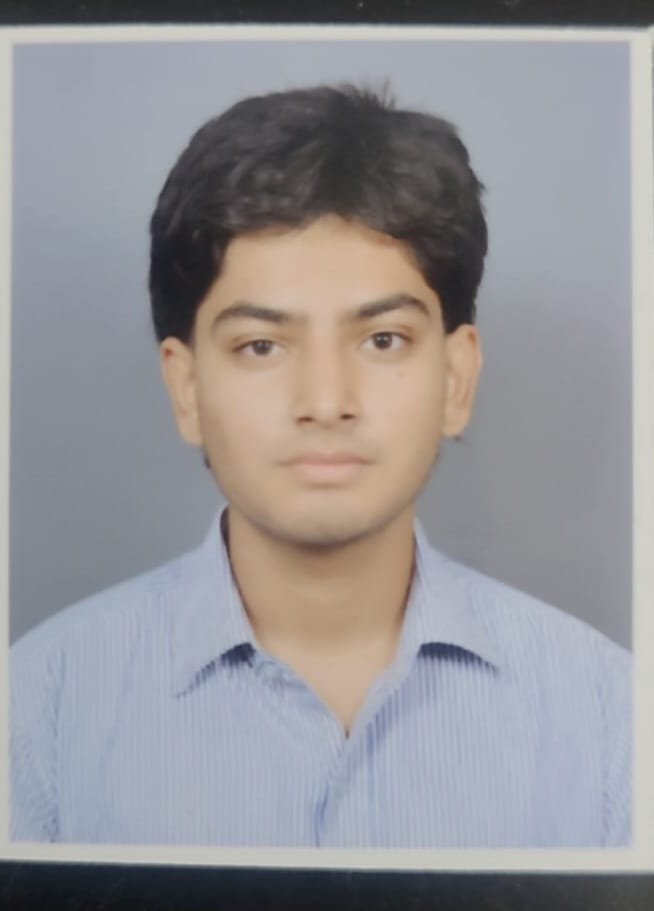
\includegraphics[width=2.0cm,height=2.3cm,keepaspectratio]{kartikey.jpeg}
\end{minipage}
\\
\hline

\begin{minipage}[t][2.6cm][c]{\linewidth}
\vspace{1.5mm}
\textbf{Team member 4}\\[-1mm]
\end{minipage}

&
\begin{minipage}[t][2.6cm][c]{\linewidth}
\vspace{1.5mm}
\textit{Md Musharaf Shah -- 2519146}\\
\textit{Section DS2}
\end{minipage}

&

\begin{minipage}[t][2.6cm][c]{\linewidth}
\centering
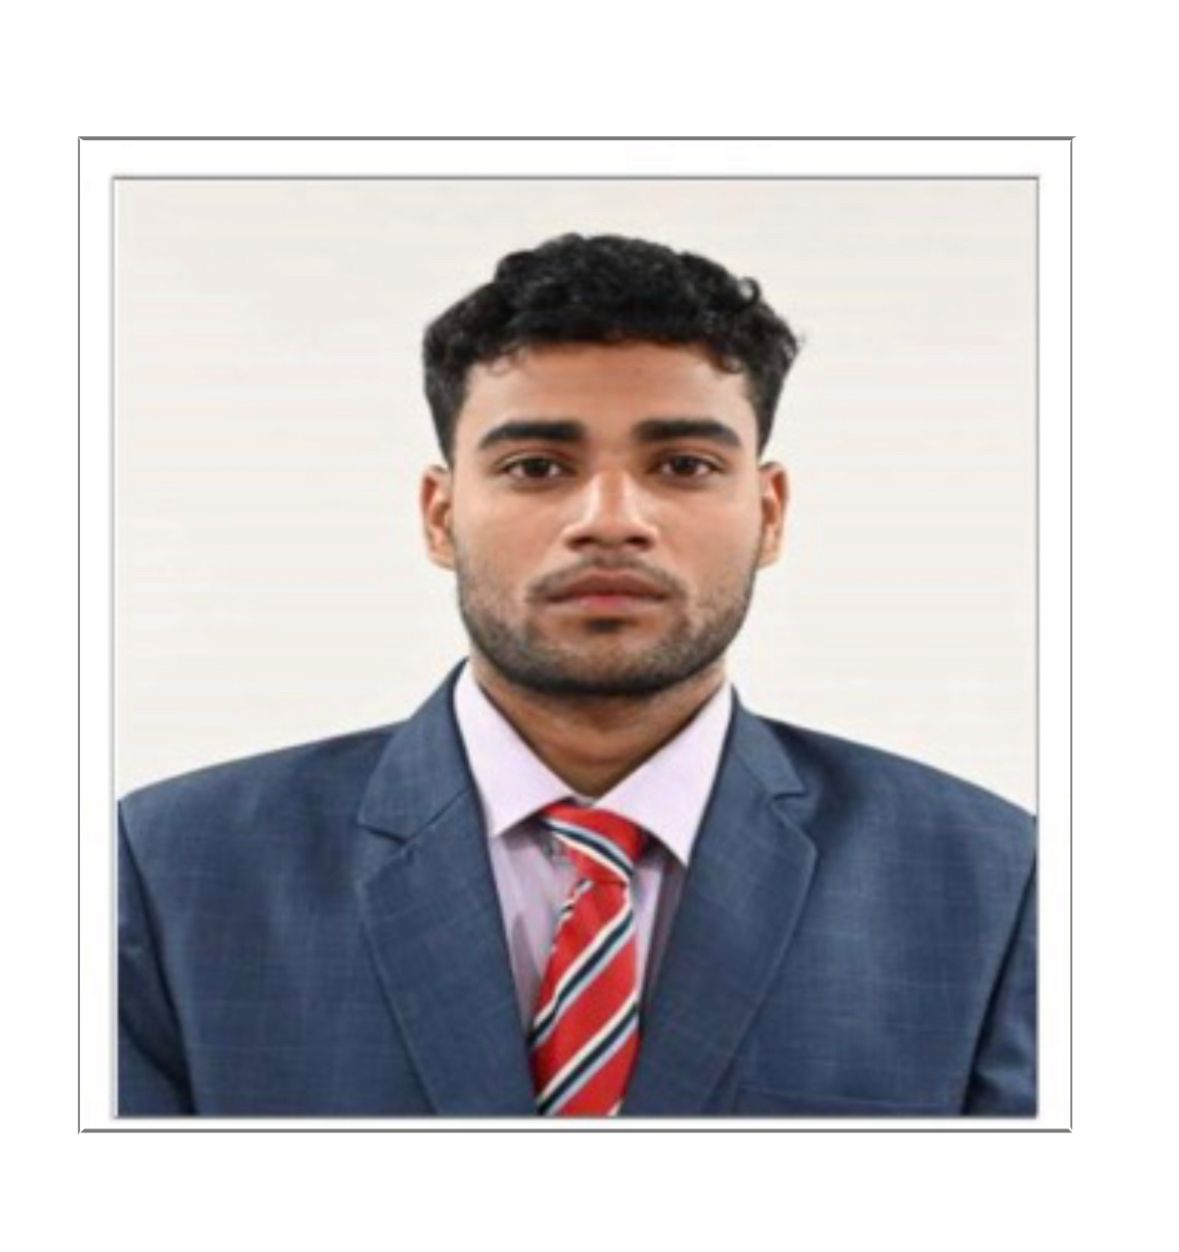
\includegraphics[width=2.0cm,height=2.3cm,keepaspectratio]{mussharaf.jpeg}
\end{minipage}
\\
\hline
\end{tabularx}

\newpage


\vspace{6mm}
\bluebigheading{PROPOSAL DESCRIPTION }

\vspace{6mm}

\blueheading{Motivation }

\vspace{1mm}


\answerbox[3.6cm]{Hospitals must simultaneously manage two competing needs: attending to patients based on medical urgency rather than arrival order, and retrieving patient or doctor records quickly even as the dataset grows large. Naive approaches such as a simple list or an unbalanced search tree fail to guarantee efficiency in either case. Delays in triaging critical patients or in locating a patient's history can have serious real-world consequences, so an efficient, well-structured management system is essential. This project designs a console-based Hospital Patient Management System that applies appropriate data structures for each sub-problem -- priority-based triage, fast lookup, and sorted record maintenance -- and evaluates their performance empirically as the number of records scales.}

\vspace{6mm}

\blueheading{State of the Art / Current solution }

\vspace{1mm}


\answerbox[3.2cm]{Many small clinics still rely on manual registers or simple FIFO-based digital queues that treat every patient identically, regardless of the severity of their condition. Basic record-keeping systems commonly use unbalanced Binary Search Trees or plain linked lists for patient data, which degrade to linear-time search as records grow or are inserted in sorted order. Larger hospital information systems use relational databases with indexing, but the underlying data-structure trade-offs (priority ordering, balanced trees, hashing) are rarely made explicit or compared, which is the gap this project addresses at a data-structures level.}

\vspace{6mm}

\blueheading{Project Goals and Milestones }

\vspace{1mm}


\answerbox[3.8cm]{\textbf{Goals:} (1) Design an object-oriented model for patients, doctors, and appointments using encapsulation, inheritance, and polymorphism. (2) Implement a priority queue for emergency triage based on severity of condition. (3) Implement a circular queue for fixed daily outpatient appointment slots. (4) Implement and compare a Binary Search Tree and an AVL Tree for maintaining sorted, searchable patient records. (5) Implement a hash table with collision resolution for near-constant-time patient lookup by ID. (6) Empirically benchmark all structures as record count increases.

\textbf{Milestones:} \emph{M1 --} Core OOP class design and file-based persistent storage with a menu-driven interface. \emph{M2 --} Circular queue and priority queue for appointment and triage handling, compared against naive FIFO ordering. \emph{M3 --} BST and AVL Tree implementation (with LL, RR, LR, RL rotations), instrumented for height and comparison counts. \emph{M4 --} Hash table implementation and consolidated benchmarking of sequential, binary, and hash-based search into a final performance report.}

\vspace{6mm}
\newpage

\blueheading{Project Approach}

\vspace{1mm}




\answerbox[3.9cm]{The system will be built as a console-based application with C used for core data-structure implementation and C++ used for the object-oriented layer. A \texttt{Person} base class will be specialised into \texttt{Patient} and \texttt{Doctor} derived classes, demonstrating encapsulation, inheritance, and polymorphism. Emergency triage will be handled by a priority queue ordered by severity, while routine outpatient slots will use a circular queue. Patient records will be maintained in both a plain Binary Search Tree and a self-balancing AVL Tree so their performance can be directly compared, and a hash table with a chosen collision-resolution strategy will provide near-constant-time lookup by patient ID. All records will be persisted using file-based storage (text/binary files). Development will use VS Code for coding and Overleaf for documentation, with each module benchmarked for height, comparison counts, and average lookup time as the dataset scales, and the results consolidated into a final performance analysis report.}

\vspace{1cm}

\blueheading{System Architecture (High Level Diagram)}

\vspace{1mm}



\answerbox[4.6cm]{\centering
\begin{tikzpicture}[
node distance=2.5mm,
layer/.style={rectangle,draw=TitleBlue,thick,fill=TitleBlue!8,minimum width=13.0cm,minimum height=0.65cm,align=center,font=\small},
comp/.style={rectangle,draw=TitleBlue,fill=white,minimum width=2.8cm,minimum height=0.55cm,align=center,font=\scriptsize},
arrow/.style={-{Stealth},thick,draw=TitleBlue}
]
\node[layer] (pres) {\textbf{Presentation Layer} --- Console Menu (UI)};
\node[layer,below=4mm of pres] (app) {\textbf{Application Layer (OOP)} --- \texttt{Person} $\rightarrow$ \texttt{Patient}, \texttt{Doctor}};
\node[comp,below=12mm of app.west,anchor=north west,xshift=1.4cm] (pq) {Priority Queue};
\node[comp,right=2.2mm of pq] (cq) {Circular Queue};
\node[comp,right=2.2mm of cq] (bst) {BST / AVL Tree};
\node[comp,right=2.2mm of bst] (ht) {Hash Table};
\begin{scope}[on background layer]
\node[layer,fit=(pq)(cq)(bst)(ht),inner sep=2.5mm] (dslayer) {};
\end{scope}
\node[font=\scriptsize\bfseries,TitleBlue,anchor=south east] at ([xshift=-1mm,yshift=0.8mm]dslayer.north east) {Data Structure Layer};
\node[layer,below=7mm of dslayer] (store) {\textbf{Persistence Layer} --- File-based Storage (Text/Binary Files)};
\draw[arrow] (pres.south) -- (app.north);
\draw[arrow] (app.south) -- (dslayer.north);
\draw[arrow] (dslayer.south) -- (store.north);
\end{tikzpicture}}

\vspace{6mm}

\blueheading{Project Outcome / Deliverables }

\vspace{1mm}


\answerbox[3.1cm]{A working console-based Hospital Patient Management System covering patient registration, emergency triage, appointment scheduling, and record retrieval. Empirical evidence that AVL trees maintain logarithmic search time even under adversarial (sorted) insertion order, while plain BST performance degrades toward linear time. A quantified comparison of emergency response ordering using a priority queue versus FIFO handling. A comparative table of search technique (sequential, binary, hash-based) versus average lookup time across varying dataset sizes, along with the complete project report and source code.}


\newpage
\vspace{6mm}

\blueheading{Assumptions}

\vspace{1mm}


\answerbox[2.9cm]{The system is developed and evaluated as a single-user, console-based application rather than a networked, multi-user system. Patient severity levels for triage are assumed to be assigned manually by staff at registration time. Dataset sizes used for benchmarking are simulated/synthetic rather than real hospital records, and storage is limited to local text/binary files rather than a full database server.}

\vspace{1cm}

\blueheading{References}

\vspace{1mm}


\answerbox[3.1cm]{1. Course syllabus, Data Structures and OOPs.\\
2. R. Kruse et al., \emph{Data Structures and Program Design in C}, Pearson Education Asia.\\
3. Herbert Schildt, \emph{The Complete Reference C++}, Tata McGraw-Hill.}

\end{document}
